\documentclass[runningheads]{llncs}

\usepackage[T1]{fontenc}

\usepackage{graphicx}

\usepackage[colorlinks,bookmarksopen,bookmarksnumbered,citecolor=blue, linkcolor=blue, urlcolor=blue]{hyperref}

\usepackage[utf8]{inputenc}

\begin{document}
	\title{A Brief Study on the Development of Predictive Process Monitoring}
	\subtitle{Seminar(IN0014) - scientific methods \\ in information systems}
	\author{Shuaiwei YU \inst{1} }
	\institute{Technical University of Munich\\
	\email{shuaiwei.yu@tum.de}}
	\maketitle
	
	%here begins the abstract
	\begin{abstract}
		Predictive process monitoring (PPM) is a powerful tool in business logic, and it is gaining more and more attention from industry and academia. Due to the great interest in this topic, a significant number of works are continuously published. Therefore there is an indispensable need to perform a literature review on predictive process monitoring. The main objective of this paper is to research the current situation and algorithmic trend of predictive process monitoring so that potential research gaps can be identified. The objective is achieved through a systematic literature review aimed at the search period of 2018 - 2022 on the topic of predictive process monitoring. A Multi-step filtering was performed on the 263 retrieved articles, and a final list of 32 papers was selected. The data subtracted from the papers are then used to analyze and summarize. The final result reveals the current trend and identifies the research gaps in PPM.

		\keywords{predictive process monitoring  \and literature review \and algorithm.}
	\end{abstract}
	
	%the first part: Introduction into the topic
	\section{Introduction}
		Predictive Process Monitoring (PPM) or Predictive Business Process Monitoring (PBPM) is known as a specific branch of process mining. Process mining focuses on the optimization of business processes using the analysis of deviation detection and the process model discovered by analyzing the historical event logs \cite{art-8}. In contrast, predictive monitoring makes predictions about the development of uncompleted business instances at runtime with given input data \cite{original}. For example, whether the customer will accept the offer, what is the next activity that will occur in a business process, or how much time it would take for the entire business pipeline to finish. 
	
		%benefits of PPM
		Implementing the PPM technique into the business logic of a firm can be very beneficial. With the support of the continuous prediction of future events, the company can provide the customer with better service quality and thus increase their competence. Predictive process monitoring is quite essential for Customer Relationship Management (CRM) by providing the prediction of the possibility of whether a customer's order will be completed on time. PPM is also an effective tool for Enterprise Resource Planning (ERP), e.g., By providing the prediction of the resources required in the next activity, the company can optimize the resource usage \cite{art-13}. The article \cite{art-29} shows us that the prediction of the remaining time is also crucial. It is necessary to communicate the prediction of the remaining time until the process completion and to provide the related partners or customers with progress information.   
		
		%some examples of advantage of PPM
		Various works already suggest the use case and the advantage of implementing predictive process monitoring. The work of \cite{art-6}, and \cite{art-7} both suggest the significant meaning of the PPM providing information on predicted failures and deviations. The work \cite{art-13} and \cite{art-24} shows how PPM can provide the managers with insights into system development and offer necessary information for CRM or ERP systems. \cite{art-5} illustrate how the analysts can intervene proactively in a business process with the prediction information.
	
		%Meaning of the event logs
		Since the PPM technique is a branch of the process mining technique, it also requires event logs as input \cite{art-15}. Nowadays, different types of information systems are already widely adopted by firms to manage workflows, plan resource allocation and manage the customer relationship. Such information systems usually produce many event logs, which provide the basic data for predictive process monitoring \cite{art-5}. The graph below demonstrates a simple example of an event log fragment. As we can see, an event log is understood as a collection of a series of \textit{traces} (they are also sometimes referred to as \textit{cases}). A trace consists of one or several events, which have a unique id to differ one from another. The ID sometimes is denoted as $ e_{n} $ with $ n \in$ |event ID|. An event is a minimum element of an event log, representing a single execution of an activity. An event can have several attributes; in our case, for example, the timestamp. 
		
		\begin{figure}
		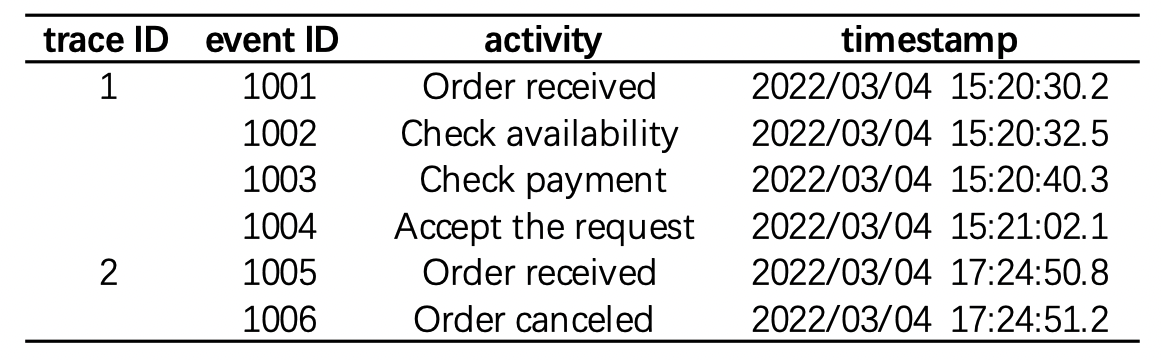
\includegraphics[scale=0.4]{event_logs.png}
		\centering
		\caption{A simple fragment of an event log} 
		\end{figure}
	
		%motivation
		As demonstrated in \cite{original}, a significant amount of literature about predictive process monitoring techniques is becoming available in recent years. A large number of articles on this topic led to the necessity to research the current situation of the PPM technique, what efforts are made, and what is the current research gaps in this field.	In this research paper, I want to answer the main research question \textbf{RQ}: "\textit{What is the development and trend of the predictive process monitoring techniques over the research period?}". This question is achieved by a systematic literature review under the guidance given by \cite{guideline}. I selected 32 papers from 263 papers, which were acquired through searching using google scholar with proper keywords. These 32 papers were then categorized, analyzed, and summarized. As a result, I identified several popular algorithms that are being used most frequently, and I also noticed some new uprising algorithmic trends nowadays. Furthermore, I also detected some potential research gaps in the current predictive process monitoring field. 
	
		The remainder of this article is developed as follows. Section 2 recorded the systematic literature review protocol, section 3 reveals the results of systematic literature review, section 4 searches on the trend of predictive process monitoring, and section 5 makes a conclusion about the article. 
	
	%the second part: Systematic Literature Review Protocol
	\section{Systematic Literature Review Protocol}
		%overview of the literature review.
		The research questions are formulated in the systematic literature review protocol, the search protocol is defined, and the selection criteria are developed. The selection criteria are based on the selection criterion of \cite{original} and are modified following the guideline provided in Kitchenham's article \cite{guideline}. The work consisted of several stages. In the first stage, The review protocol was designed. Specifically, the research questions to be investigated were formulated, and I chose the electronic database that will be used to run the search. The selection criteria, as well as inclusion criteria, were also defined. In the next stage, the horizontal search was run. The documents acquired were then filtered according to selection criteria; in the end, the final list of documents will be generated.
		
		%research questions development.
		The main research question (\textbf{RQ}): "\textit{What is the development and trend of the predictive process monitoring techniques over the research period?}" can be decomposed in four sub-question as follows. The first two sub-questions are so developed in order to research the current trends and algorithmic distribution of the predictive process monitoring. \textbf{RQ1}: "\textit{What is the distribution of the literature about predictive process monitoring over the search period?}" and \textbf{RQ2}: "\textit{What aspects can be predicted by the predictive process monitoring?}". The next sub-question focuses on the aspects of outcome that can be predicted, \textbf{RQ3}:"\textit{What is the distribution of the algorithms used in predictive process monitoring over the search period?}". In the last question, I want to research the reason that leads to the current trend of predictive process monitoring, i.e., \textbf{RQ4}: "\textit{What leads to the trend of predictive process monitoring?}"
		
		%motivations of the research questions.
		In the first research question, I want to visualize the distribution of the article published in order to analyze the current trend of predictive process monitoring. With this visualization, people are able to take a deeper look into the development of interest in the industry of predictive process monitoring. The second research question examines the distribution of algorithms used for predictive process monitoring. The motivation for this is that I want to reveal which algorithms are more popular and widely used. With the first two research questions, current research trend of predictive process monitoring can be derived. I can also analyze the possible research gaps where further academic contributions could be made. In \cite{original}, several aspects were already listed. However, the third research questions want to research whether there are new predictive aspects developed or how the new predictive process monitoring model predicts these aspects differently. The last research question tries to look into the reason that led to the current development of predictive process monitoring so that I might predict what the research direction of this field might be.
		
		%development of search string
		To develop the search string, I followed the guidelines and suggestions given by \cite{guideline} and, based on the work of \cite{original}, developed the search string I'm going to use. After defining the search string, I decided to use Google Scholar as the electronic database for its completeness and simple operability. The search period was between the years 2018 and 2022.
		
		%steps of filtering below
		The first step of the filtering is about identifying the duplicates. My goal is to identify the literature that appeared more than once and whose name and author are identical. Only one of the papers will be preserved for future processes. In the next step, I look into the title of the papers gathered. In this step, (i) the studies that are related to a different field will be removed (e.g., "A Chemical Monitoring and Prediction System in Semiconductor Manufacturing Process Using Bigdata and AI Techniques", or "Condition monitoring and prediction of solution quality during a copper electroplating process"); (ii) the documents which are not proper research papers should also be removed (e.g., "Integration of an Explainable Predictive Process Monitoring System into IBM Process Mining Suite (Extended Abstract)").
				
		%The last steps of filtering
		Moreover, I only consider the papers published in conferences, journals, and workshops, because, in comparison to degree thesis, published articles are more professional and have a higher academic contribution. In the next step of filtering, I looked into the abstract of each paper in order to evaluate its relevance. In the last stage, I use the inclusion criterion \textit{"the study should propose a novel algorithm or technique for predictive process monitoring"} to further select the papers used for our study.
		
		%clarification of the table
		The Figure \ref{Filtering} below  summarizes a specific list of my literature search. Out of 263 hits, I performed the filtering as listed above-mentioned, and according to selection criteria, I selected 28 papers. 4 more articles were added via vertical search. \footnote{The queries were run on 18th May 2022}
		
		%extraction of information of the data 
		From the final 32 papers, I extracted the meta-Information. Information about the publication date was extracted to answer \textbf{RQ1}. Every article usually comes up with an algorithm that predicts some or several aspects of the business process. Thus, I categorize each paper with its prediction level and algorithms so that the \textbf{RQ2} and \textbf{RQ3} can be answered. By analyzing the data and looking into each paper, \textbf{RQ4} in the end can be addressed.\footnote{The selected documents were visualized as an excel sheet and is available at \url{https://tumde-my.sharepoint.com/:x:/g/personal/shuaiwei_yu_tum_de/Ef8ufzITCHpNi32om-3FQUQBZvOeGkWU9LLN_ZlcvawoRQ?e=cc8cnW} }
		
		\begin{figure}
		
\includegraphics[width=\textwidth]{Filtering.png}
		\caption{Overview of Systematic Literature Review Protocol} 
		\label{Filtering}
		\end{figure}
		
		
		
	\section{Systematic Literature Review Results}
		
		%publication distribution
		To answer \textbf{RQ1}, I analyzed the publication date from the extracted meta-data by plotting the publication number. More and more publications on predictive process monitoring can be observed. Such a trend would imply that the PPM is gaining more and more attention, and the topic is becoming hotter. There is only one publication from 2022, probably because the queries were performed in May, and some papers are not yet published. Several conferences about Information Systems are not yet held, e.g., \textit{International Conference on Process Mining (ICPM)} will take place in October 2022. \footnote{\url{https://icpmconference.org/2022/}} 
		
	
		\begin{figure}
		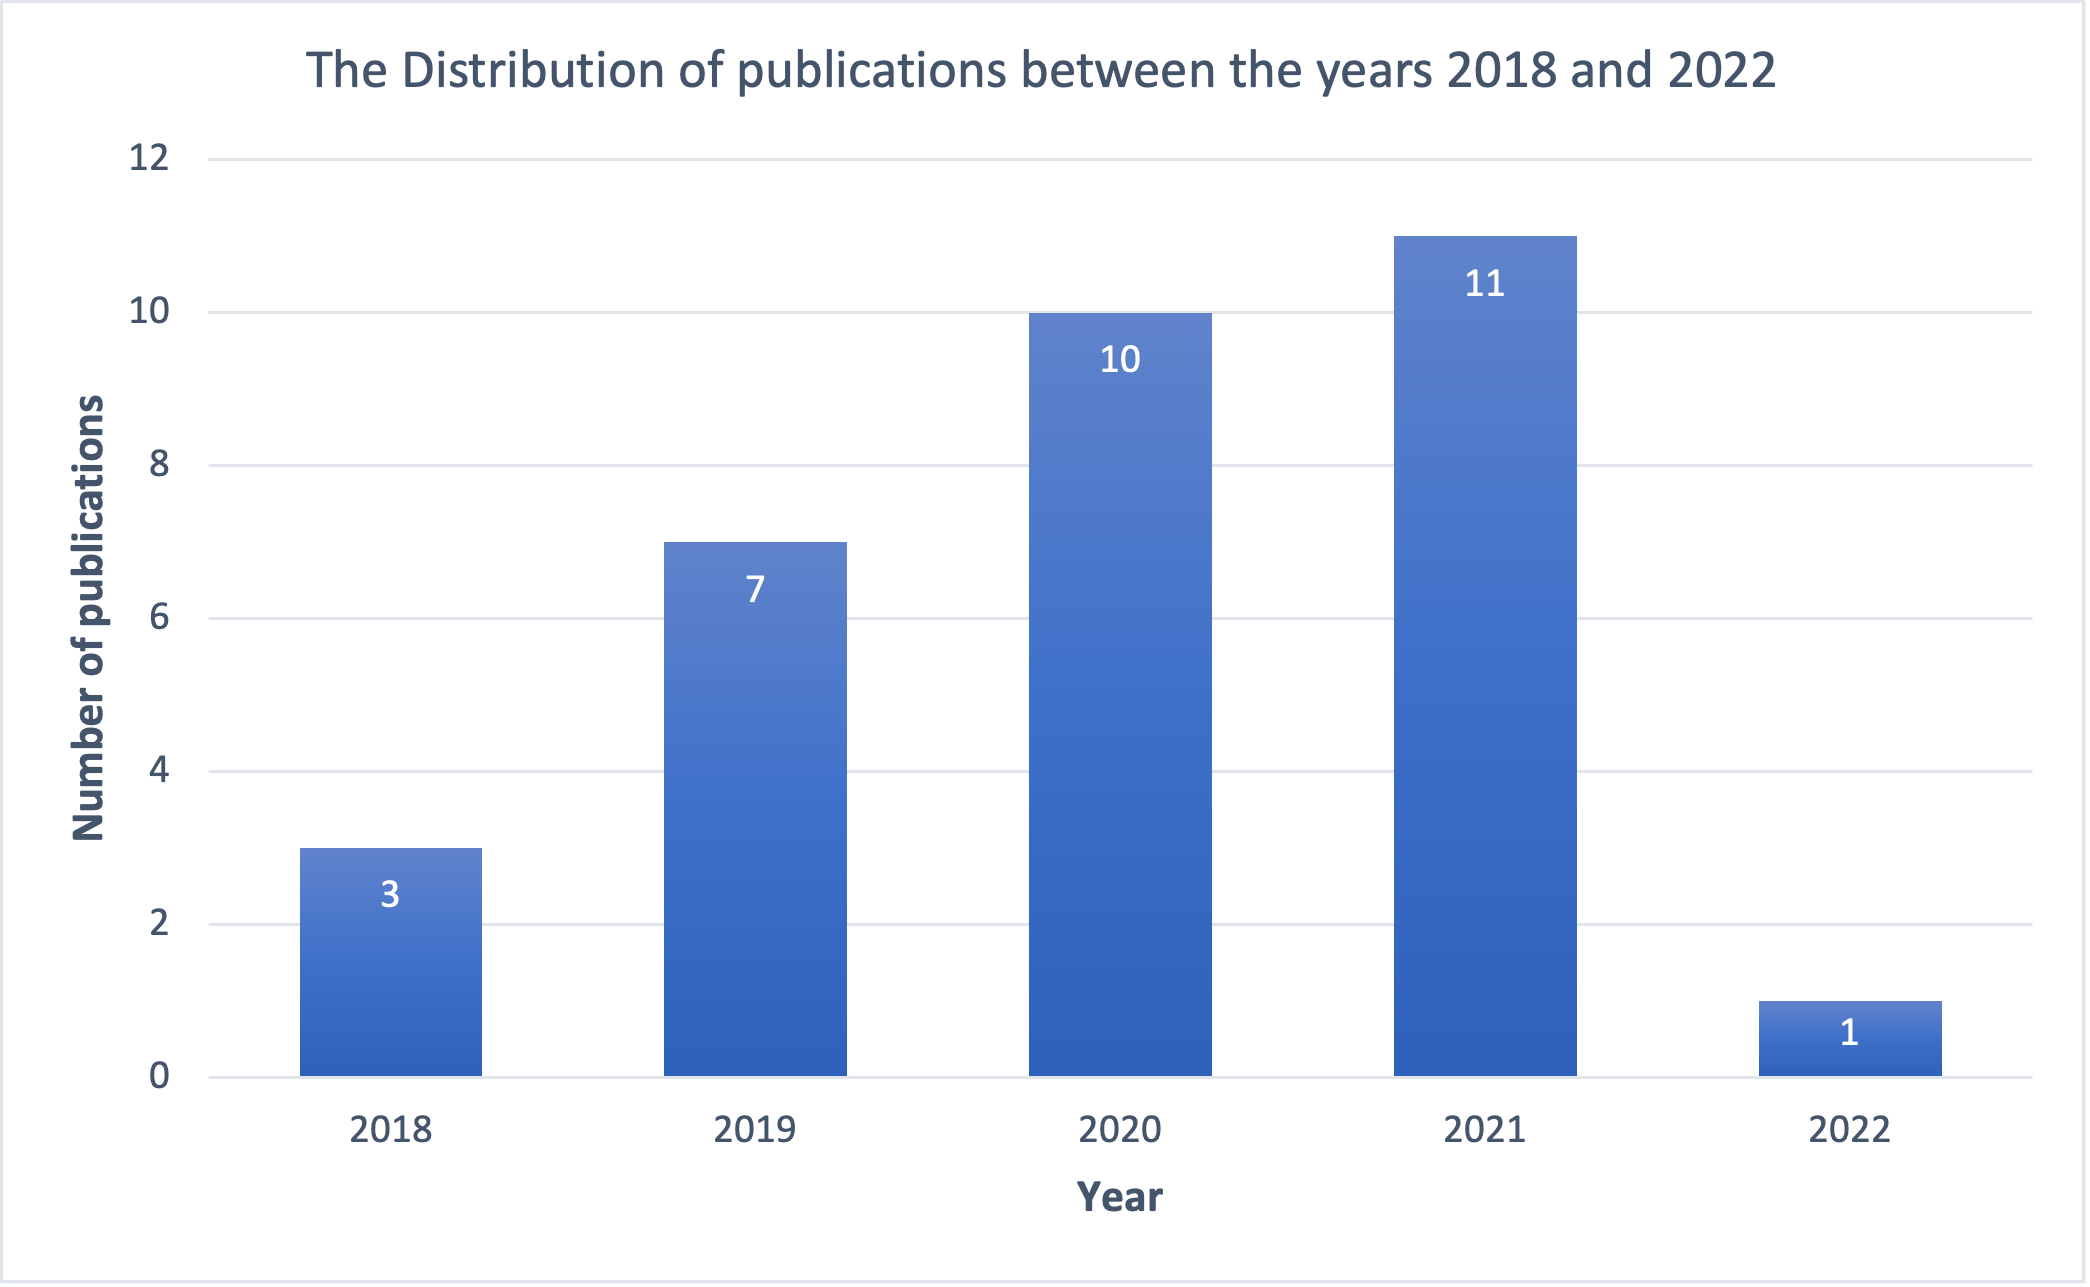
\includegraphics[scale=0.35]{Distribution_publications.png}
		\centering
		\caption{The Distribution of publications between the years 2018 and 2022}
		\end{figure}
		
		%Prediction level proportion
		To address \textbf{RQ2}, I need to look closely at the prediction level proposed in each paper. The work of \cite{original} categorized three prediction levels, i.e., Numeric Predictions,   Categorical Predictions, and Next Activities Predictions. Here I followed the same principle and categorized my final article. I calculated the proportion of each prediction level and plotted the following graph.
		
		
		\begin{figure}
		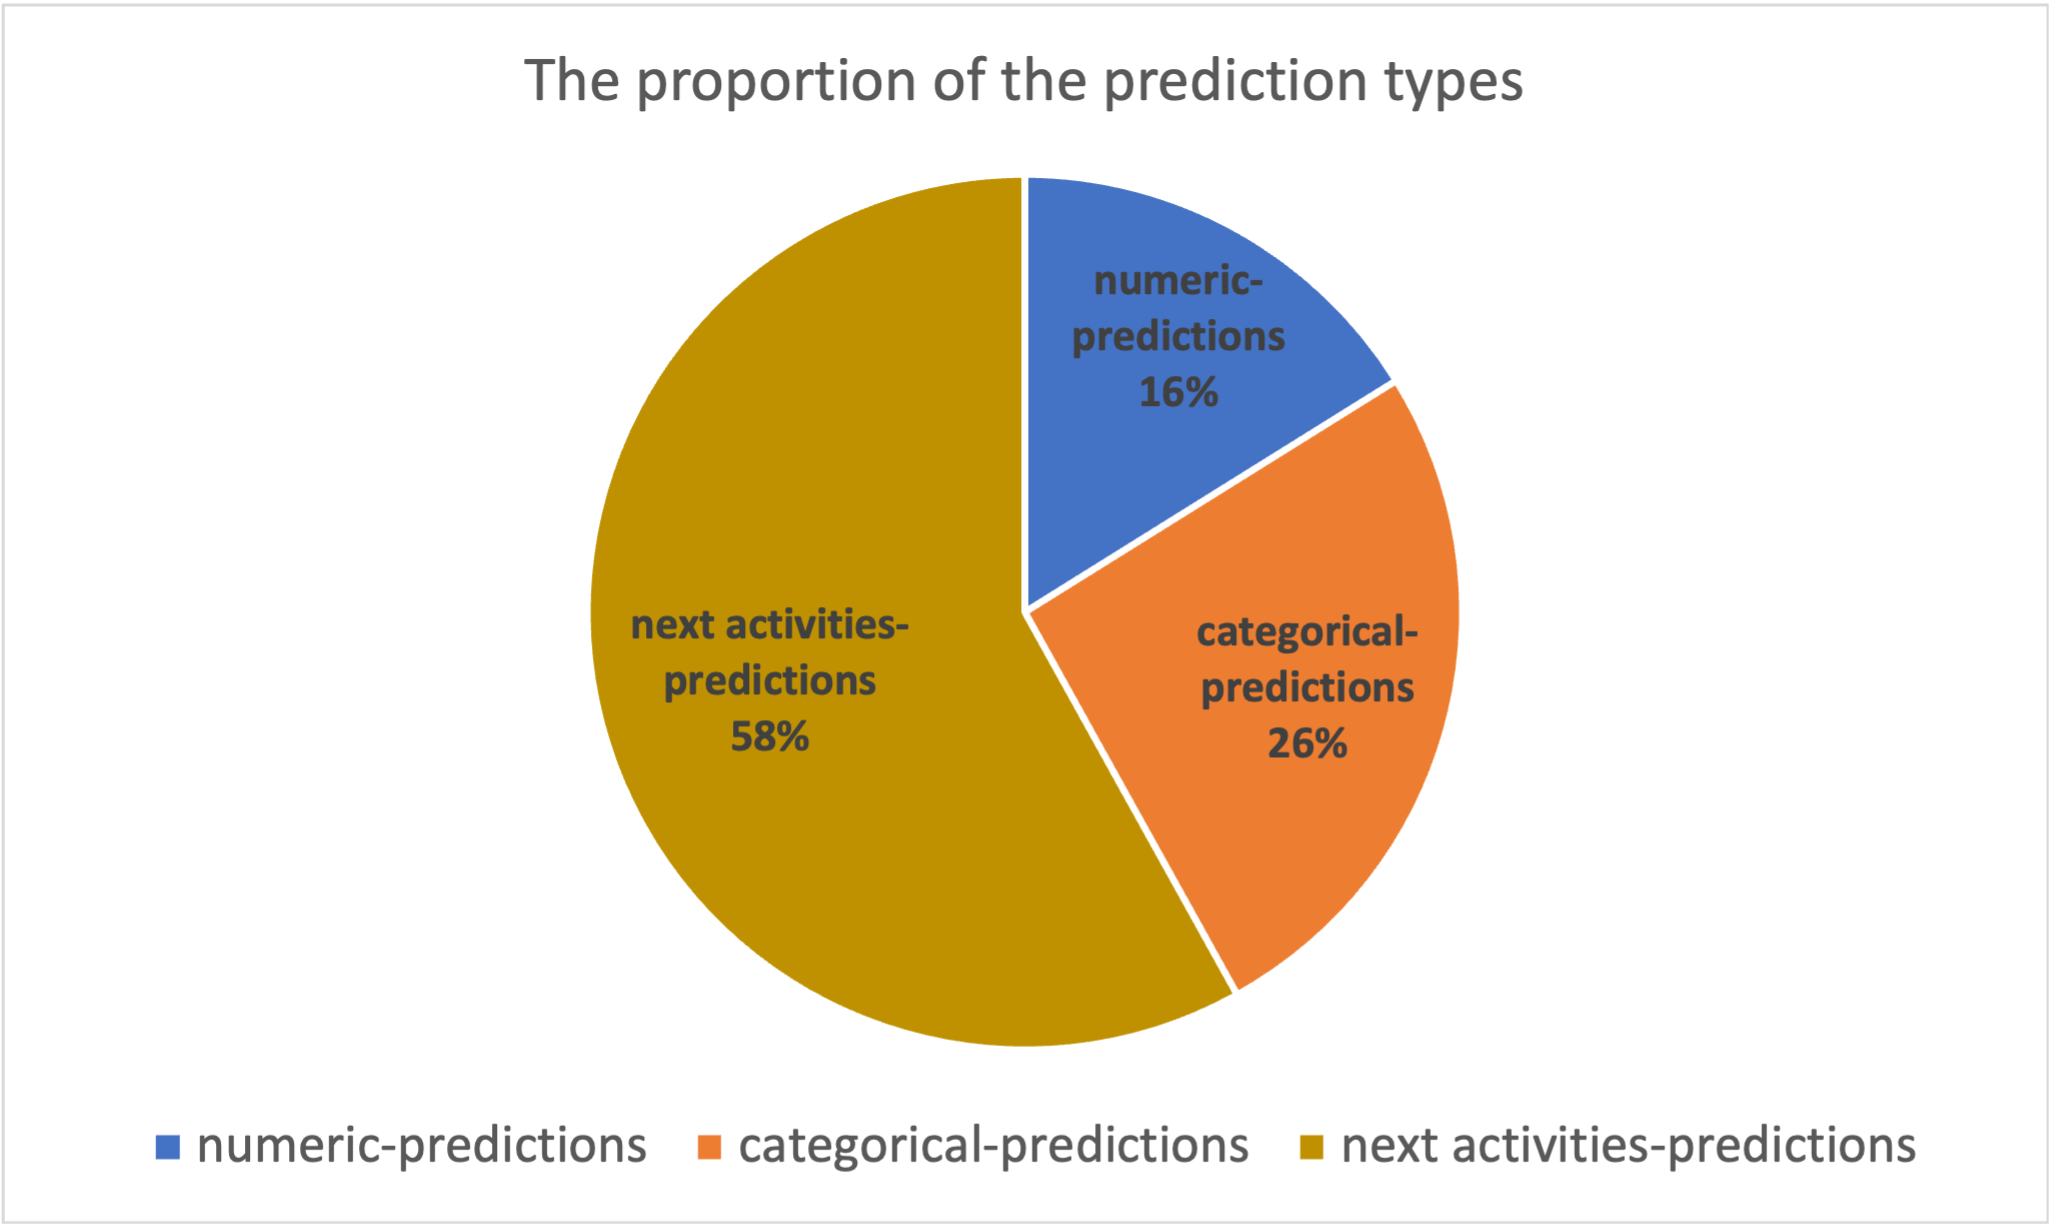
\includegraphics[scale=0.4]{proportion_prediction.png}
		\centering
		\caption{The proportion of the prediction types}
		\end{figure}
		
		People can observe that 58\% of techniques make a next-activity prediction. On the contrary, only 16\% of techniques make numeric predictions; I will look into this phenomenon in the following sub-sections. I will also summarize the benefits each prediction type brings to business logic as well as briefly talk about the algorithms' usage and new trends emerged in current studies.
		
		\subsection{Next Activities Predictions}
		The first prediction type I discovered is the next activities prediction. It predicts the next outcome or the sequence of future activities based on the already occurred events\cite{original}. As we observed from the graph above, most of the predictive process monitoring techniques make the next activities prediction. In \cite{art-5} and \cite{art-24}, the authors argue that the next activities prediction is a fundamental problem because analysts can act proactively with the prediction information to prevent undesired behaviors and guarantee higher utilization. \cite{art-18} also suggests that the prediction information can be used as the prerequisite of subsequent checks. The reason why people are so interested in the next activities prediction is worth discussing. \cite{art-7} already issued the concern of undesired deviations. Such deviations from workflow routines or deadline violations are problematic because they will cause irreparable costs and time waste in firms. Therefore, it is indispensable to identify and notify about deviations before they occur so that preventive measures can be undertaken. 
		
		The research in recent years proposed fascinating new insights and advanced novel algorithms to develop the next activities prediction model. \cite{art-5} \cite{art-7} \cite{art-14} \cite{art-23} \cite{art-24} \cite{art-28} \cite{art-31} all used neural networks to propose their models. However, they implemented the neural networks differently. \cite{art-5} proposes a model that combines deep learning and multi-view learning. \cite{art-7} leverages the attention mechanism from Natural Language Processing. Using an attention mechanism, instead of the final layer in the neural network constructing the context vector, every hidden state participates, improving prediction accuracy. In \cite{art-14}, the authors exploit the information from the elapsed time between events and thus propose a PBPM model based on time-aware LSTM cells. \cite{art-23} and \cite{art-24} use the convolutional neural networks architecture to address the problem. Machine learning is another popular algorithm family used in this prediction type. \cite{art-1} combined global and local prediction techniques. Global techniques consider historic behavior at once, while local prediction techniques concentrate on some specific subsets of the historic process behavior. \cite{art-25} and \cite{art-30} build Dynamic Bayesian Networks. Bayesian Network is a probabilistic model revealing the relationships of random variables in a complicated model. Dynamic Bayesian Network is a subclass of Bayesian Network. Because the contextual information in predictive process monitoring changes dynamically, implementing Dynamic Bayesian Networks can be beneficial. \cite{art-10} use the Markov chain models. Depending only on the current state, Markov chain model is a statistical model to evaluate systems concerning the future. The authors of \cite{art-30} believe that the next event prediction is insufficient. Instead, they used machine learning models to develop a KPI system to recommend next best actions.
		
		\subsection{Categorical Predictions}
		The second prediction type is the categorical prediction. The predictions about the categorical outcome and risk monitoring are made. \cite{art-9} claims that the outcome prediction represents a run-time process most intuitively. The outcome prediction can be summarized as problems of classification given input in the early stage; The example for this prediction type can be very intuitive, e.g., in the service branch, whether the customer is satisfied with the solution or the service provided; In the business area, this technique can be used to predict whether a purchase order will be successfully closed or will be withdrawn, or the ordered products will be delivered on time \cite{art-12}.
	
		Several families of algorithms are used in the prediction family. A new technique that emerged in recent years also draws my attention -- Explainable AI (XAI). Several papers about the XAI are used in the categorical predictions to find the explanations for the classification predictions made by the models and try to enhance people's trust in the PPM techniques. 
		
		\cite{art-4} and \cite{art-26} leverage the traditional machine learning methods to develop the prediction model. However, the specific algorithm being used is different. The authors of \cite{art-4} argue that Bayesian Networks (BN) are under-explored and come up with two approaches based on Bayesian Networks to handle the uncertainty in PPM. The first approach utilizes parameter learning in BN, which is suitable when facing the lack of the event logs or the business process is complex; In the second approach, parameters and the BN's structure are directly learned by the event log. \cite{art-26} applied cost-sensitive learning (CSL) to address the problem of predicting non-frequent trace variants. The concept of CSL is to assign misclassification cost to each class, and the ML model tries to minimize the total misclassification cost. CSL can capture rare activities of particular importance to increase prediction accuracy. \cite{art-8} focuses on exploiting the latent factors in the event logs, for example, policies, laws, biases, etc. \cite{art-9}, and \cite{art-12} here leverage the neural network technique again to make the prediction. On the one hand, \cite{art-9} combined the LSTMs model with the attention mechanism and proposed a new effective model called  Att-Bi-LSTM by introducing the idea of natural language process. On the other hand, \cite{art-12} is inspired by the achievement in computer vision, and the authors introduce the concept in computer vision into process mining by associating similar trace values with neighbor pixel frames. \cite{art-9} address the issues of traditional models such as random forest, i.e., the models require to select tailor-made operations manually offline. As a result, different selections lead to different performances. The authors combined the attention mechanism with a BiLSTM network composed of forward LSTM and backward LSTM to build their own model. The advantage of such a model is its efficiency, and the model also has a better performance. \cite{art-12} suggests that computer vision technology can also be applied to the predictive process monitoring sector. The prefix traces are first mapped onto a vector, which will then be encoded and transformed into a 2D image representing the trace. Based on such images, a CNN architecture is finally trained. The outcome seems to be promising. 
		
		\subsection{Numeric Predictions}
		The work focuses on numeric predictions is another crucial area. However, the research papers published during the search period focus majorly on time prediction. Thus in this section, we will be concentrating only on the remaining time prediction. As demonstrated in \cite{art-13}, The prediction of the remaining time can be beneficial in areas where the scheduling and choice determination are involved. \cite{art-15} also addresses the significance of the remaining time prediction by mentioning its usage to avoid undesirable situations during the running business process. \cite{art-29} suggest that the remaining time should be communicated between business partners to provide the customer with better service. 
		
		The works in this area all rely on specific models. It is clear that different methods are used to make the prediction, but among them, neural networks are the most commonly used method. \cite{art-29} points out that the prediction of remaining execution time belongs to regression problems and \cite{art-17} illustrated that the Long Short-Term Memory networks (LSTMs) commonly perform better than other models. Due to these facts, it is not hard to imagine why neural networks are the most commonly used ones.
		
		In\cite{art-15} \cite{art-21} \cite{art-29}, neural networks are leveraged to make a precise prediction. In \cite{art-15}, the authors employed Deep Neural Network (DNN) and Entity Embedding technique to raise the predictive accuracy. Entity Embedding is important in this context to raise the speed of the neural network; this encoding method clusters the intrinsically similar values that will be denoted as vectors and placed near each other to reduce memory usage. \cite{art-21} uses LSTM neural network to implement the prediction model. \cite{art-21} suggests that LSTM overcomes the drawback of Recurrent Neural Networks (RNN), which is good at short-term sequential prediction but fails to manage long-term predictions. LSTM networks solve the problem by maintaining some aspects constant of the information flow within the neural cells. \cite{art-29} also leverages the LSTM model to perform the prediction. However, the article also proposes the goal of optimization of selecting publishing points. \cite{art-17} attempts to explain the prediction models with Explainable AI based on the game theory of Shapley Values. The Shapley value of a variable refers to the contribution of this variable to the prediction. In \cite{art-13}, the authors propose to record the spatial event log at the event log that is used as input data to increase accuracy.       

		
		\section{Research on the Algorithmic Trend}
		
		To address \textbf{RQ3}, we have to look deeper into the algorithms used in each paper. Thus I summarized the family of algorithms used throughout the research period. We can derive from this graph that the Neural Networks are dominantly used. However, the traditional machine learning methods are not yet outdated; they still find usage in recent works. In recent years, the adoption of Explainable AI in predictive process monitoring is also observed, and it could possibly bring new insights into the Process mining area.       
		
		\begin{figure}
		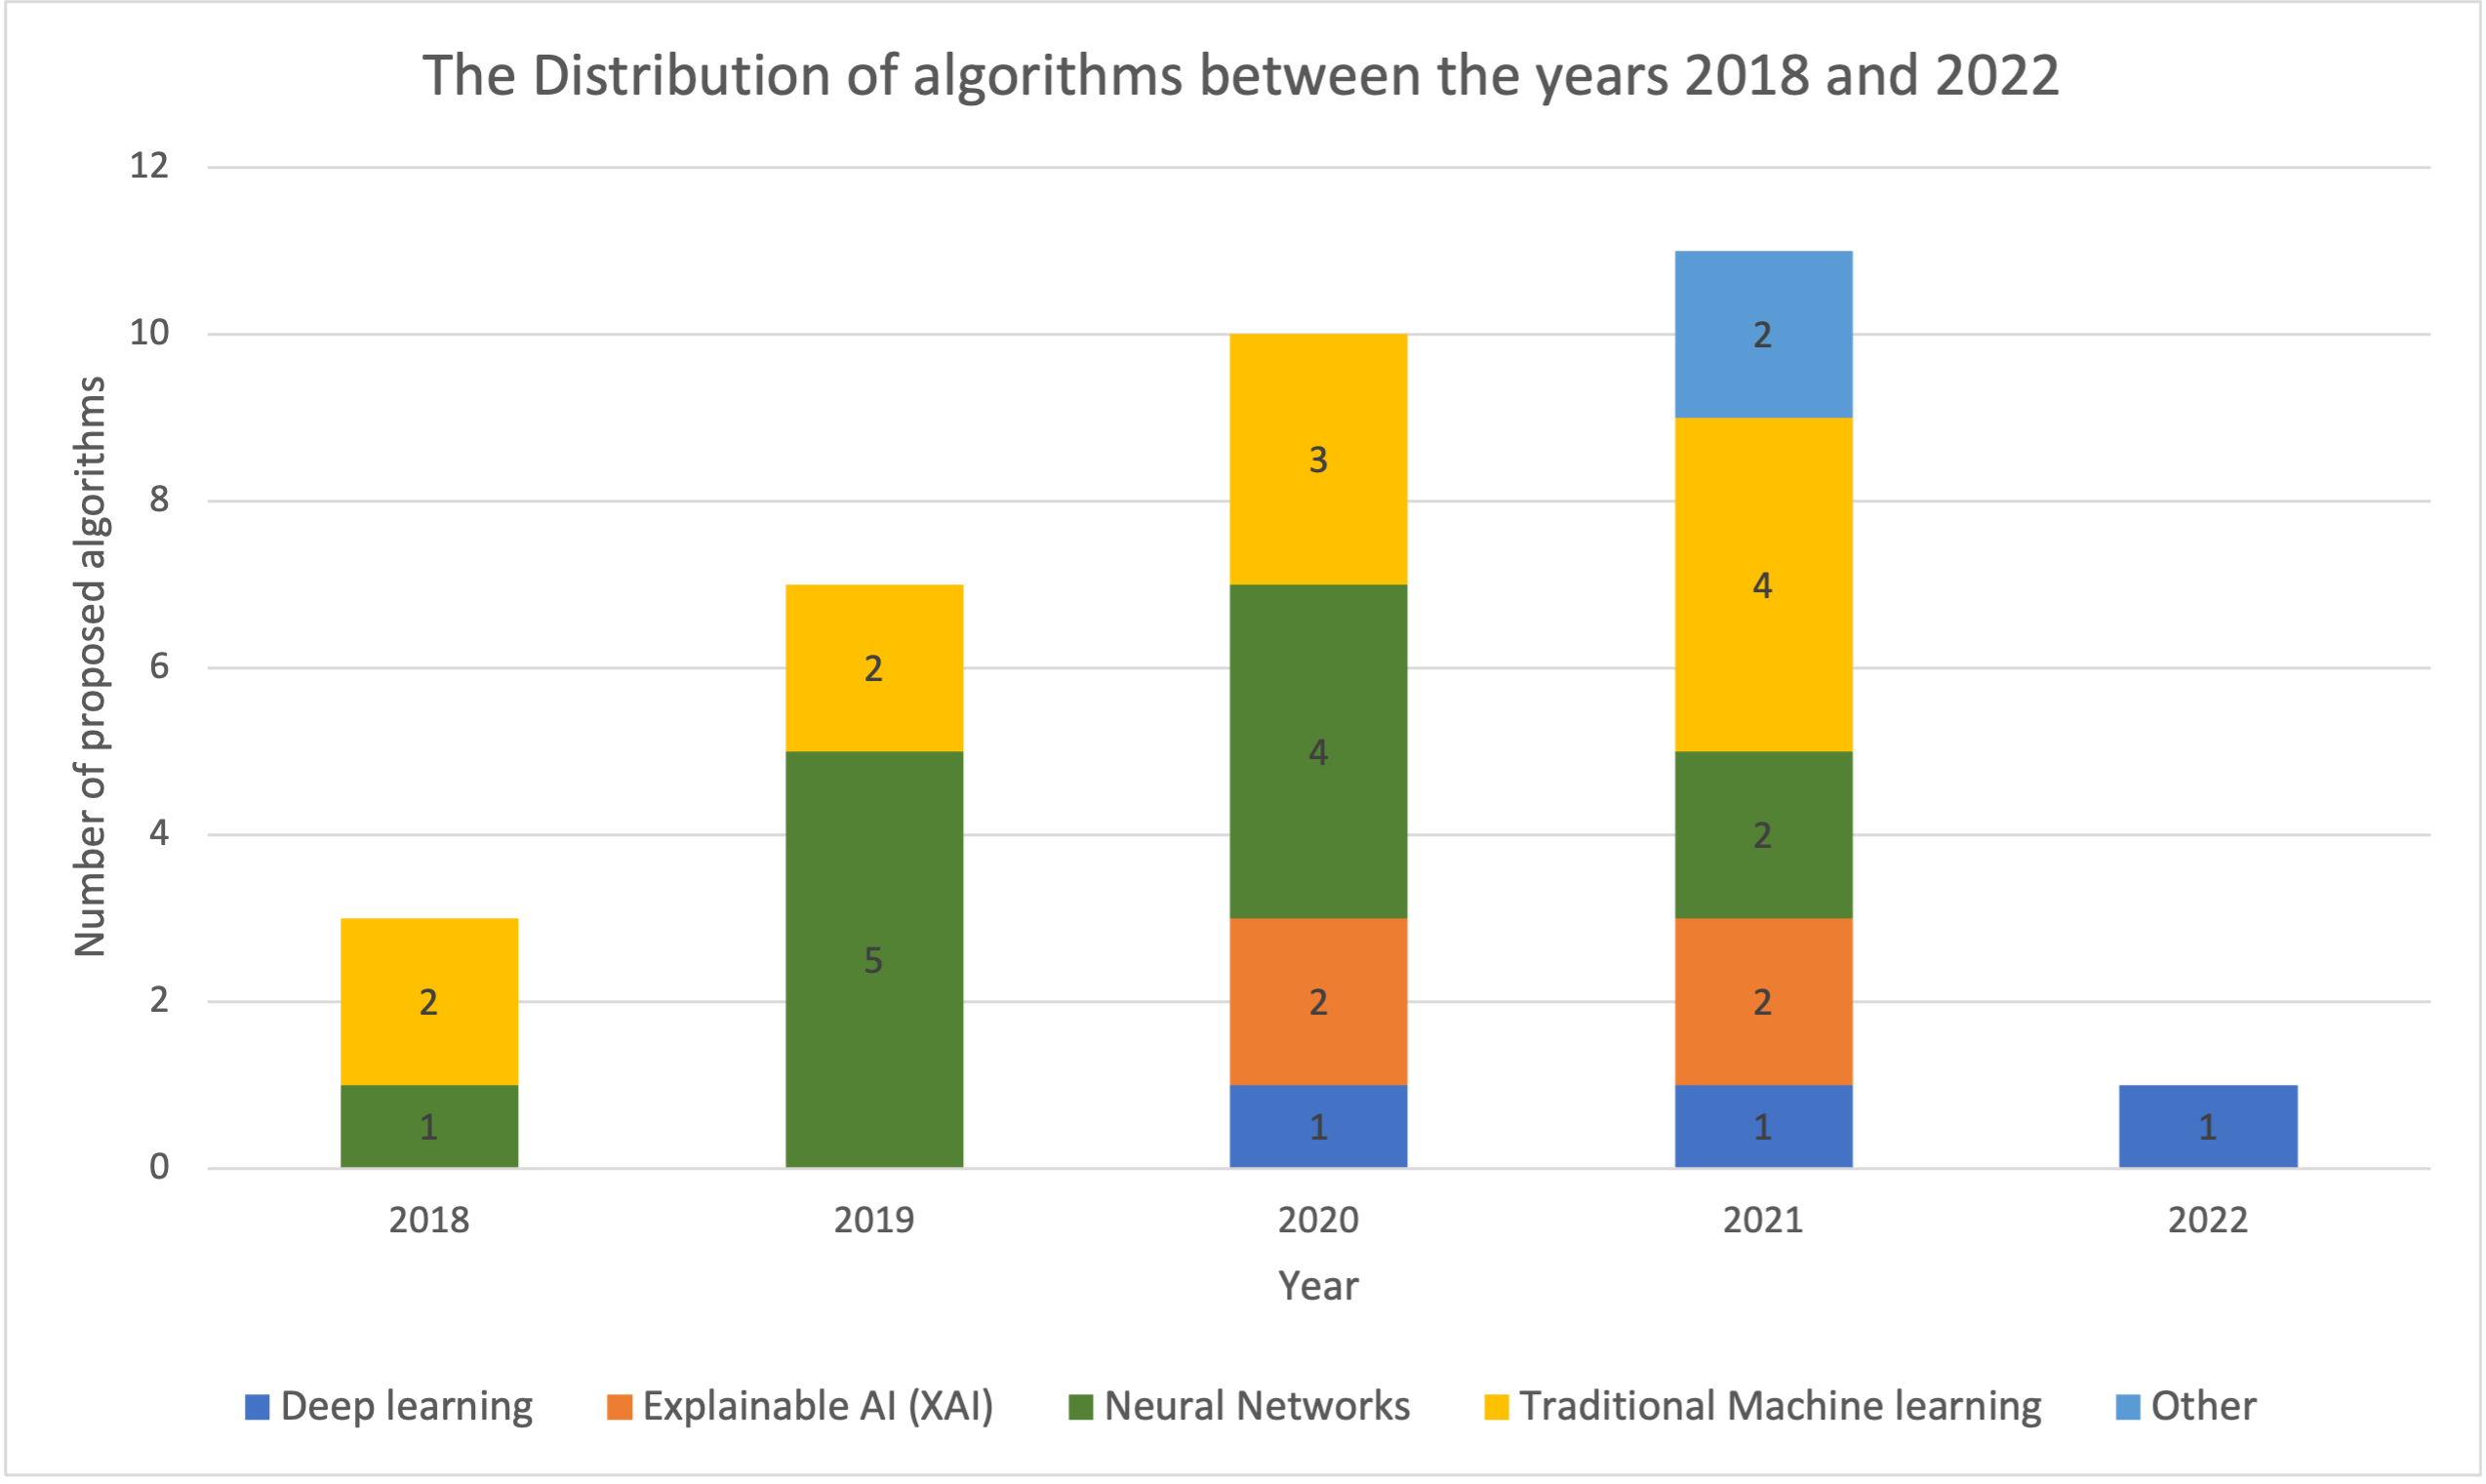
\includegraphics[scale=0.35]{Distribution_algorithms.png}
		\centering
		\caption{The Distribution of algorithms between the years 2018 and 2022}
		\label{algo1}
		\end{figure}
		
		\textbf{RQ3} now leads us to \textbf{RQ4}. It is beneficial for us to search the algorithmic trend of PPM and the reason behind this, by taking a look of this trend, we are also able to identify the new possible research gaps in the current research field. I plotted the following graph by classifying the algorithms used in each prediction type. 
		
		\begin{figure}
		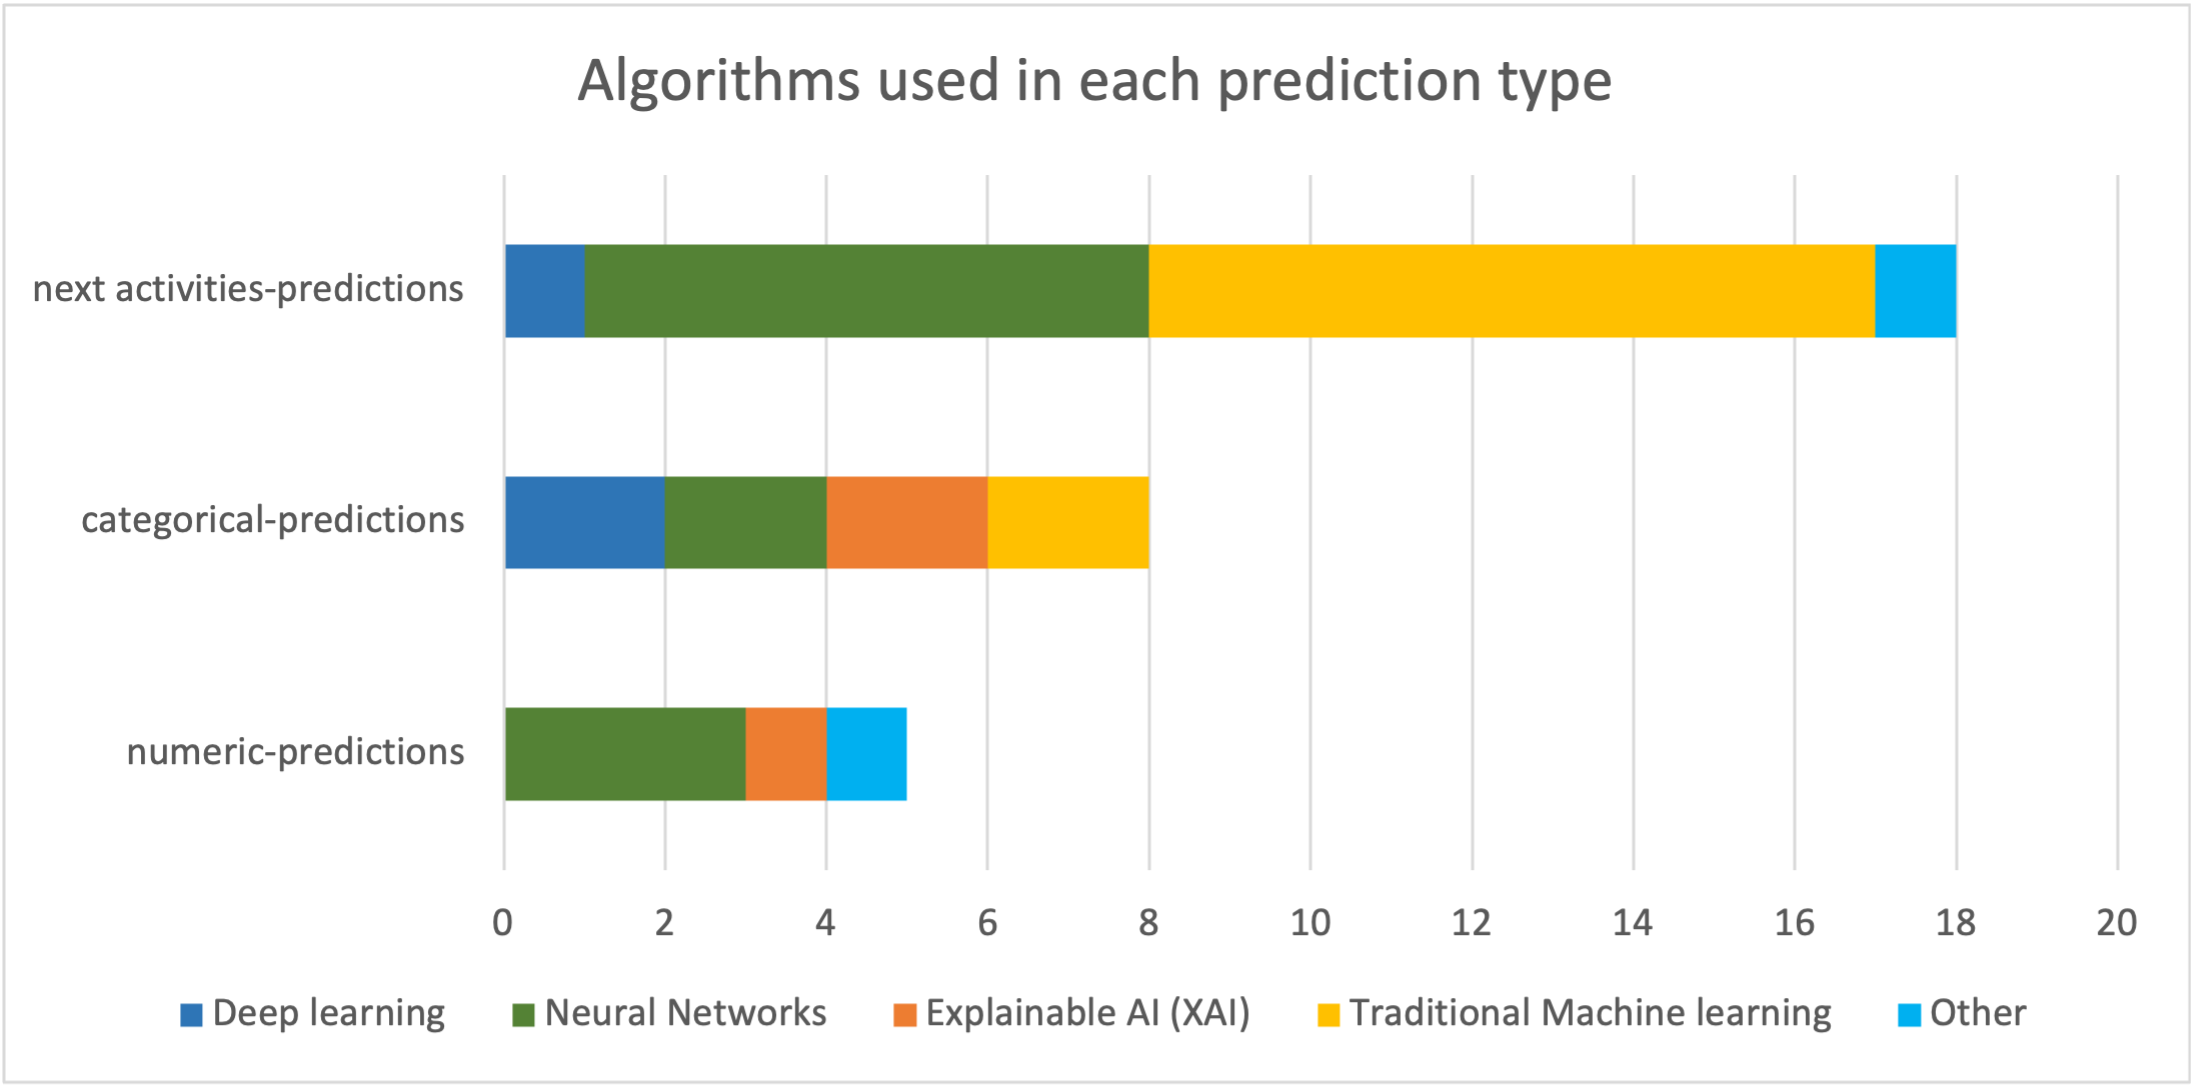
\includegraphics[scale=0.4]{Algorithms_usage.png}
		\centering
		\caption{Algorithms used in each prediction type}
		\label{algo2}
		\end{figure}
		
		As observed from the figure \ref{algo1} and \ref{algo2}, I want to talk about some most intuitive and representative algorithms from recent studies. I will also try to look into the development of the algorithms' usage.
		
		\subsection{From naïve Bayes to Bayesian Networks}
		\cite{art-6} states that the prediction of discrete target values can be considered classification problems. For instance, the outcome prediction of customer service can be classified as a binary result, either satisfied (true) or dissatisfied (false). Bayesian models drew my attention among all algorithms for classification problems in predictive process monitoring. Naïve Bayes Classifier is the most intuitive and straightforward model of the Bayesian model family. As given in \cite{slide-1} Naive Bayes classifier considers all attributes and assumes all attributes are equally important and independent. People can easily calculate the probability of a Random Variable. However, as in \cite{slide-1} addressed, adding redundant attributes is problematic for Naïve Bayes. Bayesian Network (BN) is a more advanced and powerful tool to present the probabilistic relationships of variables \cite{art-4}. BNs have several advantages, such as combining different sources of knowledge, supporting decision analysis, and fast responses. BN model is a Directed Acyclic Graph and is represented by $ G = (V, E)$, where $V$ is nodes in the graph, and it represents the considered random variables, e.g., observable quantities or latent variables. $E$ means the conditional relationships between the random variables. Every node is related to a probability function, and the function computes the node's probability with the values of this node's parent variables \cite{art-4}. Dynamic Bayesian Networks (DBNs) are a subclass of BNs that can model dynamic systems like stochastic processes. The DBN's structure and parameters are usually fixed; thus, it can be considered a network representation of a dynamic system \cite{art-25}.   		
		
		\subsection{RNN and LSTMs}
		Although the traditional machine learning method is interpretable and robust, their accuracies are usually not as high as neural networks nowadays. Therefore, researchers are paying more and more attention to models based on neural networks. I want to first talk about Recurrent Neural Networks (RNN). The basic structure of RNN is its procession of cyclical connections. Because of this particular structure, the RNN uses a part of the output produced by its predecessor. As a result, RNN performs very well in predicting sequential data \cite{art-21}. However, RNN is not efficient when dealing with long-term dependencies. In order to address this problem, Long Short-Term Memory (LSTM) networks are introduced. LSTM is based on the RNN; LSTM not only uses the output from the predecessor but also maintains long-term memory. This is achieved by maintaining some certain aspects constant during the whole process \cite{art-21}. The authors of \cite{art-9} developed a new model based on LSTM. They argue that although the LSTM network generates classifiers representing the relationship between cases and the outcome, such a relationship is very dynamic in outcome prediction. Therefore, the authors combined the forward LSTM and backward LSTM and used this as a hidden layer to extract features in the event logs. In \cite{art-14}, the researchers built Time-Aware Long Short-term Memory (T-LSTM) Cells based on the fundamental structure of LSTM. The article suggests that the primary LSTM cells assume the elapsed time between events is uniformly distributed. It is, however, rarely the case. The designed T-LSTM cells can consider irregular elapsed times when processing event logs. It is achieved by decomposing the previous cell memory. The RNN and LSTM serve as a starting point and the basis for the further implementation of predictive process monitoring models. I believe they still have much potential to be exploited.     
	
		\subsection{Explainable AI (XAI)}
		Nearly every work on Explainable AI addresses the concern of the black-box nature or state-of-the-art property of the neural network, like the LSTM models mentioned in the above section. User trust is very crucial in the business area \cite{art-17} since the prediction models usually cannot offer a convincing explanation of the generated prediction decision, people would hesitate to adopt the predictive process monitoring technique. Hence, the XAI aims to offer explanations and strengthen people's trust in the prediction model. The techniques for XAI are mostly post hoc interpretation which means after a prediction model is generated, explanations and visualizations are extracted \cite{art-20}. The work of \cite{art-17} showed us the usage of the SHAP implementation, which is based on the game theory of Shapley values. The implemented explanation model delivered us the contribution of each variable. \cite{art-20} leveraged the Local Interpretable Model-Agnostic Explanations (LIME) to explain the model by approximating it using a locally interpretable linear model. The Study of \cite{art-11} brings us even further. The article \cite{art-11} suggests that XAI can also detect the error in prediction models. Such errors are generated in the learning phase, where some data in the training set might be incorrect; thus, a perfect classifier cannot be trained. \cite{art-11} wants to identify why a classifier is mistaken and use the XAI to correct such errors to train a better classifier. The researchers find the most common features that lead the predictor to produce wrong predictions by observing the false-positive and false-negative instances in the confusion matrix. To increase accuracy, they then retrain the classifier with the information abstracted in the last step.        
				
		\
		
		As concluded above, we identified some trends of predictive process monitoring. Traditional machine learning models still perform very reliable and offer very good explainability. However, more and more attention is paid to algorithms based on neural networks because they usually offer very high accuracy. Furthermore, Explainable AI enhances people's trust in decisions made by neural networks and offers us new insights into predictive process monitoring. I also identified some research gaps in the current field. I believe researchers can pay more attention to numeric predictions because the papers published recently on this topic are still relatively few. I also think that we can bring explainable AI into all three prediction topics to let them illustrate the reason behind the prediction models. It is also possible to apply the traditional machine learning algorithms to numeric prediction for more profound research on this matter.   
		
		
		\section{Conclusion}
		The predictive process monitoring techniques have been growing and are receiving more and more attention in recent years. Such trends allow researchers and entrepreneurs to use these techniques to analyze the business process and dynamically predict the future. However, due to the increasing number of published papers, it is sometimes difficult to identify the current research trends and the potential research gaps. Through a systematic literature review in the field of predictive process monitoring, I looked into the current situation of predictive process monitoring. I discovered some trends as well as uncovered some potential research gaps.
		
		In order to achieve a thorough and comprehensive study, the bias and incompleteness of the selection for literature should be guaranteed. To achieve this, I carefully followed the guide on a literature search of \cite{guideline}. I used Google scholar to perform the search, to search as many relevant publications as possible. Furthermore, I also performed a back-ward search to conclude related articles. To increase the creditability of this work, the replication of this work is also guaranteed. However, the results could slightly vary due to the date of search and the algorithms used by databases.
		
		In future work, I plan to divide the classification of algorithm family more into details to see whether there are more algorithmic trends and connections between the predictive process monitoring. This systematic literature review can serve as a supplementary for the researchers who want to research in this field and might bring new insights and inspirations.
		
	\newpage
	\begin{thebibliography}{99}
	
	\bibitem{original}
	Di Francescomarino C, Ghidini C, Maggi F M, et al. Predictive process monitoring methods: Which one suits me best?[C]//International conference on business process management. Springer, Cham, 2018: 462-479.
	
	\bibitem{guideline}
	Kitchenham B. Procedures for performing systematic reviews[J]. Keele, UK, Keele University, 2004, 33(2004): 1-26.
	
	\bibitem{art-1}
	Böhmer K, Rinderle-Ma S. LoGo: combining local and global techniques for predictive business process monitoring[C]//International Conference on Advanced Information Systems Engineering. Springer, Cham, 2020: 283-298.
	
	\bibitem{art-2}
	Böhmer K, Rinderle-Ma S. Probability based heuristic for predictive business process monitoring[C]//OTM Confederated International Conferences" On the Move to Meaningful Internet Systems". Springer, Cham, 2018: 78-96.
	
	\bibitem{art-3}
	Weinzierl S, Zilker S, Stierle M, et al. From predictive to prescriptive process monitoring: Recommending the next best actions instead of calculating the next most likely events[C]//Wirtschaftsinformatik (Zentrale Tracks). 2020: 364-368.
	
	\bibitem{art-4}
	Prasidis I, Theodoropoulos N P, Bousdekis A, et al. Handling Uncertainty in Predictive Business Process Monitoring with Bayesian Networks[C]//2021  12th International Conference on Information, Intelligence, Systems \& Applications (IISA). IEEE, 2021: 1-8.
	
	\bibitem{art-5}
	Pasquadibisceglie V, Appice A, Castellano G, et al. A multi-view deep learning approach for predictive business process monitoring[J]. IEEE Transactions on Services Computing, 2021.
	
	\bibitem{art-6}
	Pasquadibisceglie V, Appice A, Castellano G, et al. A multi-view deep learning approach for predictive business process monitoring[J]. IEEE Transactions on Services Computing, 2021.
	
	\bibitem{art-7}
	Jalayer A, Kahani M, Beheshti A, et al. Attention mechanism in predictive business process monitoring[C]//2020 IEEE 24th International Enterprise Distributed Object Computing Conference (EDOC). IEEE, 2020: 181-186.
	
	\bibitem{art-8}
	Lu K, Fang X, Fang X. Business Process Outcome Prediction Based on Deep Latent Factor Model[J]. Electronics, 2022, 11(9): 1509.
	
	\bibitem{art-9}
	Wang J, Yu D, Liu C, et al. Outcome-oriented predictive process monitoring with attention-based bidirectional LSTM neural networks[C]//2019 IEEE International Conference on Web Services (ICWS). IEEE, 2019: 360-367.
	
	\bibitem{art-10}
	Khan N, McClean S, Ali Z, et al. Predictive process monitoring using a Markov model technique[C]//2019 International Conference on Computing, Electronics \& Communications Engineering (iCCECE). IEEE, 2019: 193-196.
	
	\bibitem{art-11}
	Rizzi W, Di Francescomarino C, Maggi F M. Explainability in predictive process monitoring: when understanding helps improving[C]//International Conference on Business Process Management. Springer, Cham, 2020: 141-158.
	
	\bibitem{art-12}
	Pasquadibisceglie V, Appice A, Castellano G, et al. ORANGE: outcome-oriented predictive process monitoring based on image encoding and CNNs[J]. IEEE Access, 2020, 8: 184073-184086.
	
	\bibitem{art-13}
	Ogunbiyi N, Basukoski A, Chaussalet T. Incorporating spatial context into remaining-time predictive process monitoring[C]//Proceedings of the 36th Annual ACM Symposium on Applied Computing. 2021: 535-542.
	
	\bibitem{art-14}
	Nguyen A, Chatterjee S, Weinzierl S, et al. Time matters: time-aware LSTMs for predictive business process monitoring[C]//International Conference on Process Mining. Springer, Cham, 2020: 112-123.
	
	\bibitem{art-15}
	Wahid N A, Adi T N, Bae H, et al. Predictive business process monitoring–remaining time prediction using deep neural network with entity embedding[J]. Procedia Computer Science, 2019, 161: 1080-1088.
	
	\bibitem{art-16}
	Mehdiyev N, Fettke P. Explainable artificial intelligence for process mining: A general overview and application of a novel local explanation approach for predictive process monitoring[J]. Interpretable Artificial Intelligence: A Perspective of Granular Computing, 2021: 1-28.
	
	\bibitem{art-17}
	Galanti R, Coma-Puig B, de Leoni M, et al. Explainable predictive process monitoring[C]//2020 2nd International Conference on Process Mining (ICPM). IEEE, 2020: 1-8.
	
	\bibitem{art-18}
	Rico P, Cuadrado F, Dueñas J C. Online Model Generation for Scalable Predictive Process Monitoring[C]//2021 International Young Engineers Forum (YEF-ECE). IEEE, 2021: 7-12.
	
	%\bibitem{art-19}
	%Pauwels S, Calders T. Incremental predictive process monitoring: The next activity case[C]//International Conference on Business Process Management. Springer, Cham, 2021: 123-140.
	
	\bibitem{art-20}
	Ouyang C, Sindhgatta R, Moreira C. Explainable AI Enabled Inspection of Business Process Prediction Models[J]. arXiv preprint arXiv:2107.09767, 2021.
	
	\bibitem{art-21}
	Camargo M, Dumas M, González-Rojas O. Learning accurate LSTM models of business processes[C]//International Conference on Business Process Management. Springer, Cham, 2019: 286-302.
	
	\bibitem{art-22}
	Appice A, Di Mauro N, Malerba D. Leveraging shallow machine learning to predict business process behavior[C]//2019 IEEE International Conference on Services Computing (SCC). IEEE, 2019: 184-188.
	
	\bibitem{art-23}
	Mauro N D, Appice A, Basile T. Activity prediction of business process instances with inception CNN models[C]//International conference of the italian association for artificial intelligence. Springer, Cham, 2019: 348-361.
	
	\bibitem{art-24}
	Pasquadibisceglie V, Appice A, Castellano G, et al. Using convolutional neural networks for predictive process analytics[C]//2019 international conference on process mining (ICPM). IEEE, 2019: 129-136.
	
	\bibitem{art-25}
	Brunk J, Stierle M, Papke L, et al. Cause vs. effect in context-sensitive prediction of business process instances[J]. Information Systems, 2021, 95: 101635.
	
	\bibitem{art-26}
	Käppel M, Jablonski S, Schönig S. Cost-sensitive predictive business process monitoring[C]//European Conference on Advances in Databases and Information Systems. Springer, Cham, 2021: 14-26.
	
	\bibitem{art-27}
	Weinzierl S, Dunzer S, Tenschert J, et al. Predictive business process deviation monitoring[C]//Proceedings of the 29th European Conference on Information Systems (ECIS). 2021.
	
	\bibitem{art-28}
	De Smedt J, De Weerdt J, Mori J, et al. Predictive Process Model Monitoring using Recurrent Neural Networks[J]. arXiv preprint arXiv:2011.02819, 2020.
	
	\bibitem{art-29}
	Jian C, Xiaofu H, Qing Q. Selecting Publishing Points for the Optimal Sharing of Predictive Monitoring Information of a Service Process[C]//2019 IEEE International Conference on Web Services (ICWS). IEEE, 2019: 368-372.
	
	\bibitem{art-30}
	Brunk J, Revoredo K, Stierle M, et al. Prediction of Business Process Instances with Dynamic Bayesian Networks[C]//SIMPDA. 2018: 50-54.
	
	\bibitem{art-31}
	Taymouri F, Rosa M L, Erfani S, et al. Predictive business process monitoring via generative adversarial nets: the case of next event prediction[C]//International Conference on Business Process Management. Springer, Cham, 2020: 237-256.
	
	\bibitem{art-32}
	Sikaroudi A M E, Rahman M H. Predictive process mining by network of classifiers and clusterers: the PEDF model[J]. arXiv preprint arXiv:2011.11136, 2020.
	
	\bibitem{slide-1}
	Martin, B. (2021) 'Naïve Bayes and Bayes Networks' [Lecture], IN2028: Business Analytics and Machine Learning. Technical University of Munich. 18 November.
		
	\end{thebibliography}

	
\end{document}
